%%%%%%%%%%%%%%%%%%%%%%%%%%%%%%%%%%%%%%%%%%%%%%%%%%%%%%%%%%%%%%%%%%%%%%%%%%%
%% This file is part of the book
%%
%% Algorithmic Graph Theory
%% http://code.google.com/p/graph-theory-algorithms-book/
%%
%% Copyright (C) 2009--2011 Minh Van Nguyen <nguyenminh2@gmail.com>
%%
%% See the file COPYING for copying conditions.
%%%%%%%%%%%%%%%%%%%%%%%%%%%%%%%%%%%%%%%%%%%%%%%%%%%%%%%%%%%%%%%%%%%%%%%%%%%

\documentclass{article}

\usepackage{tikz}
\usetikzlibrary{external}
\tikzexternalize{component-density-lattice}

\begin{document}

\begin{figure}
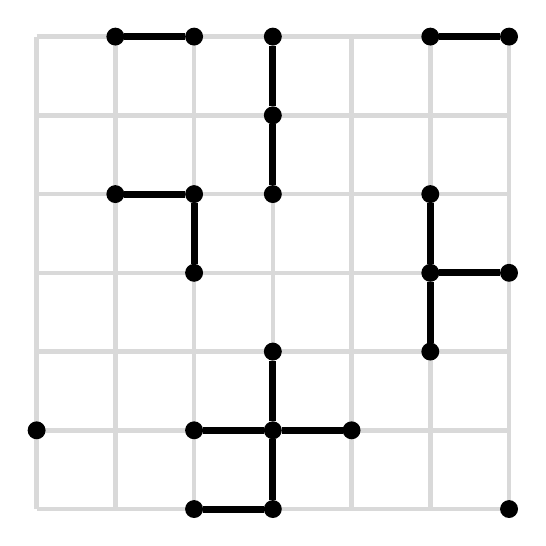
\begin{tikzpicture}
[blackFilled/.style={shape=circle,fill=black,inner sep=2pt,draw,thick},%
  darkLine/.style={line width=2.5pt},%
  lightLine/.style={-,ultra thick,color=gray!30}]
%% set up the grid
\foreach \xstart/\xend/\y in {0/6/0, 0/6/1, 0/6/2, 0/6/3, 0/6/4, 0/6/5, 0/6/6}
{
  \draw[lightLine] (\xstart,\y) -- (\xend,\y);
  \draw[lightLine] (\y,\xstart) -- (\y,\xend);
}
%% draw the nodes
\foreach \nodename/\x/\y in {01/0/1, 14/1/4, 16/1/6, 20/2/0, 21/2/1,
  23/2/3, 24/2/4, 26/2/6, 30/3/0, 31/3/1, 32/3/2, 34/3/4, 35/3/5,
  36/3/6, 41/4/1, 52/5/2, 53/5/3, 54/5/4, 56/5/6, 60/6/0, 63/6/3,
  66/6/6}
{
  \node (\nodename) at (\x,\y) [blackFilled] {};
}
%% draw the edges
\foreach \u/\v in {
  %% horizontal edges
  20/30, 21/31, 31/41, 53/63, 14/24, 16/26, 56/66,
  %% vertical edges
  23/24, 30/31, 31/32, 34/35, 35/36, 52/53, 53/54}
{
  \draw[darkLine] (\u) -- (\v);
}
\end{tikzpicture}
\end{figure}

\end{document}

\end{document}
